%%%%%%%%%%%%%%%%%%%%%%%%%%%%%%%%%%%%%%%%%%%%%%%%%%%%%%%%%%%%%%%%%%%%%%%%%%%%%%%%
%2345678901234567890123456789012345678901234567890123456789012345678901234567890
%        1         2         3         4         5         6         7         8

\documentclass[letterpaper, 10 pt, conference]{ieeeconf}  % Comment this line out if you need a4paper

%\documentclass[a4paper, 10pt, conference]{ieeeconf}      % Use this line for a4 paper

\IEEEoverridecommandlockouts                              % This command is only needed if 
                                                          % you want to use the \thanks command

\overrideIEEEmargins                                      % Needed to meet printer requirements.

% See the \addtolength command later in the file to balance the column lengths
% on the last page of the document

% The following packages can be found on http:\\www.ctan.org
%\usepackage{graphics} % for pdf, bitmapped graphics files
%\usepackage{epsfig} % for postscript graphics files
%\usepackage{mathptmx} % assumes new font selection scheme installed
%\usepackage{times} % assumes new font selection scheme installed
%\usepackage{amsmath} % assumes amsmath package installed
%\usepackage{amssymb}  % assumes amsmath package installed



\usepackage{amsmath,amssymb}

\usepackage{tikz,hyperref,graphicx,units,subfig}
\usepackage{benktools}

\usepackage{sidecap,wrapfig}
\usepackage[ruled,vlined]{algorithm2e}
\DeclareMathOperator*{\argmin}{arg\,min}
\DeclareMathOperator*{\argmax}{arg\,max}
\newcommand{\abs}[1]{\lvert#1\rvert} 
\newcommand{\norm}[1]{\lVert#1\rVert}
%\newcommand{\suchthat}{\mid}
\newcommand{\suchthat}{\ \big|\ }
\newcommand{\bd}{\mathbf{d}}
\newcommand{\bn}{\mathbf{n}}
\newcommand{\bp}{\mathbf{p}}
\newcommand{\bw}{\mathbf{w}}
\newcommand{\by}{\mathbf{y}}
\newcommand{\bx}{\mathbf{x}}
\newcommand{\bz}{\mathbf{z}}
\newcommand{\bbf}{\mathbf{f}}
\newcommand{\bzero}{\mathbf{0}}
\newcommand{\bG}{\mathbf{G}}
\newcommand{\bA}{\mathbf{A}}
\newcommand{\bW}{\mathbf{W}}
\newcommand{\bX}{\mathbf{X}}
\newcommand{\mX}{\mathcal{X}}
\newcommand{\mD}{\mathcal{D}}
\newcommand{\mN}{\mathcal{N}}
\newcommand{\mW}{\mathcal{W}}
\newcommand{\mF}{\mathcal{F}}
\newcommand{\bZ}{\mathbf{Z}}

\newcommand{\bfc}{W}
\newcommand{\Qinf}{Q_{\infty}}
\newcommand{\st}[1]{_\text{#1}}
\newcommand{\rres}{r\st{res}}
\newcommand{\pos}[1]{(#1)^+}
\newcommand{\depth}{\operatorname{depth}}
\newcommand{\dist}{\operatorname{dist}}
\newcommand{\convhull}{\operatorname{ConvexHull}}
\newcommand{\minksum}{\operatorname{MinkowskiSum}}



\title{\LARGE \bf
Multi-Armed Bandit Models for Sample-Based Grasp Planning in the Presence of Uncertainty [v-13 09-30-2014]}


\author{Michael Laskey, Zoe McCarthy, Jeff Mahler, Florian T. Pokorny, Sachin Patil,\\ Jur Van Den Berg,  Danica Kragic, Pieter Abbeel, and Ken Goldberg}% <-this % stops a space

\newtheorem{theorem}{Theorem}

\begin{document}



\maketitle
\thispagestyle{empty}
\pagestyle{empty}


%%%%%%%%%%%%%%%%%%%%%%%%%%%%%%%%%%%%%%%%%%%%%%%%%%%%%%%%%%%%%%%%%%%%%%%%%%%%%%%%


\begin{abstract}
Gaussian Process Implicit Surface (GPIS) have emerged recently as a new probabilistic shape representation.  Former methods for grasp evaluation with shape uncertainty require sampling from  distributions on shape. Given a GPIS model this would mean sampling from the signed distance field in a uniform grid of side length $n$.  The computational complexity of this operation is $O(n^6)$ in 2D and $O(n^9)$ in 3D. We propose an alternative to sampling from shape distributions and demonstrate how this reduces the computational complexity to $O(n^3)$ in both 3D and 2D for evaluation of a single grasp. We furthermore introduce the idea of adaptive sampling in the context of choosing the best grasp given a set of grasps and a GPIS object model by formulating it as a budgeted multi-arm bandit problem. We show an order of magnitude reduction in the number of samples needed vs. a non-adaptive approach and we have statistical guarantees with our method. 
\end{abstract}
%%%%%%%%%%%%%%%%%%%%%%%%%%%%%%%%%%%%%%%%%%%%%%%%%%%%%%%%%%%%%%%%%%%%%%%%%%%%%%%%
\section{Introduction}

\vspace{10pt}

\todo{Get High res GPIS visualizations, Incorporate next round of feedback}
Consider a robot packing boxes in a shipping warehouse environment. The robot will frequently encounter objects that it has not seen before. The robot will have to plan stable grasps without any prior information other than its sensor data. As seen in Fig. \ref{fig:noisy data}, with today's RGB and depth sensors, surface properties, such as specularity and transparency, can greatly effect the returned observations. Grasp planners based on deterministic algorithms are not designed to handle such noise and could fail. To plan grasps in a partially observed world, recent research has focused on incorporating uncertainty in the shape of the object \cite{kehoe2012estimating}, \cite{christopoulos2007handling}, \cite{zheng2005}.

A common method to evaluate a grasp with uncertainty is to perform Monte-Carlo integration on a grasp evaluation method. Methods to evaluate a grasp can either be a physics based algorithm \cite{ferrari1992}\cite{pokorny2013classical} or actually trying the grasp in simulation \cite{miller2004graspit} \cite{73}. Since, Monte-Carlo integration requires many evaluations to reach convergences this can be a very computationally intensive operation, when dealing with the problem of choosing the best grasp to select. We show that by framing this problem as a multi-arm bandit problem \cite{barto1998reinforcement}, we can intelligently select which grasps to sample from and  have shown empirically to find the best grasp an order of magnitude faster than a simple uniform sampling policy using only the simplest methods from this field. 

\begin{figure}[ht!]
\centering
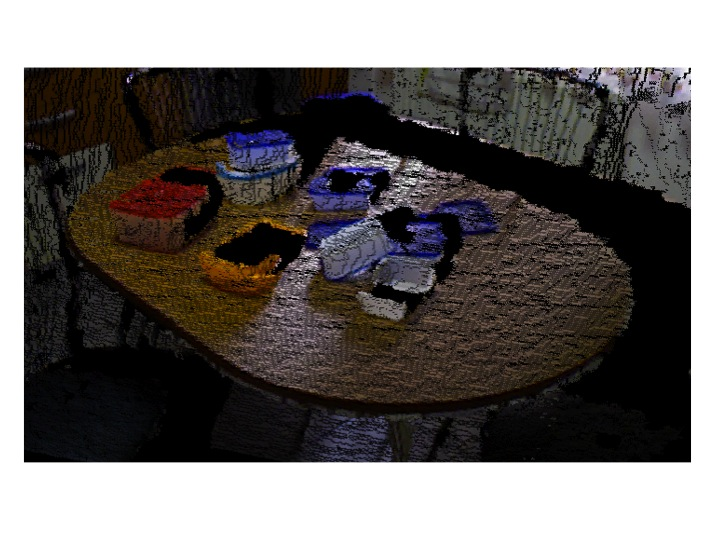
\includegraphics[width=8.5cm,height=4cm]{figures/Slide02.jpg}
\caption{\footnotesize
Left: HD image of a common measuring cup from in a household environment. Right: Image taken from PR2's Primesense Carmine sensor, large parts of the measuring cup are not detected by the depth sensor and are not visible in the RGB image.}
\vspace*{-10pt}
\label{fig:noisy data}
\end{figure}



We apply our multi-arm bandit approach to an emerging new representation in shape uncertainty, the Gaussian Process Implicit Surface, which puts a Gaussian prior on signed distance fields.  The signed distance fields (SDFs), is a continuous valued function that is an implicit surface: zero-valued at the surface of the object, positive value outside the surface and negative valued inside the surface. This representation is growing in popularity in the robotics field for its ability to integrate range data in real time \cite{newcombe2011kinectfusion}, \cite{curless1996volumetric}. To incorporate uncertainty one can use a Gaussian Process Implicit Surface (GPIS), a Gaussian process over signed distance field. Not only does GPIS present a straightforward and formal way to incorporate measurements from visual, laser and tactile sensors, they  also allow for a continuous differentiable function on shape, which can be used for a feedback grasp controller, finding locally optimal grasps and active exploration  \cite{dragiev2011}, \cite{jeffs}, \cite{hollinger2013}. 
 

Given a method to represent shape uncertainty a policy for grasp sampling, we still need to draw samples from a distribution to evaulate a grasp.  A common technique is to sample from the distribution on shape and calculate the quality of grasp on that shape\cite{kehoe2012estimating}, \cite{kehoe2012toward}, \cite{christopoulos2007handling}. Applying this technique to GPIS requires an exhaustive sampling of the signed distance field, which scales $O(n^6)$ for a 2D $n \times n$ workspace and $O(n^9)$ for a 3D workspace.The computationally complexity of sampling is derived from the fact sampling from a Gaussian requires matrix inversion of the entire signed distance field. Our paper reduces this complexity to $O(n^3)$ by using the insight that for grasp quality evaluation one only cares about the parameters that define a grasp: contacts points, surface normals, center of mass and friction coefficient \cite{pokorny2013classical}. We constrain the contact points by considering the approach trajectory of a gripper.  Hence, sampling the whole signed distance field is not needed, but instead one can only work with the distributions on grasp parameters given the shape uncertainty model and gripper trajectory. In light of this our contributions are the following:
 
\begin{enumerate}
\item Framing the selection of a grasp as from a given set as a mutli-arm bandit problem 
	\item Derivation of  distributions on grasp parameters given GPIS shape uncertainty model and approach trajectory of gripper.
	\item  Demonstrating both theoretically and empirically how those distributions reduce the computational complexity of sampling.
	
\end{enumerate}
 
\section{Related Work}

The multi-armed bandit problem~\cite{barto1998reinforcement, lai1985asymptotically, robbins1985some} is to maximize the total expected reward over a sequence of possible choices over a set of competing options, each of which has a probabilistic reward function.
The optimal sequence of choices if the rewards are known is to always pick the option with the maximum expected reward over the set of possible options.
However, to discover which choice is optimal requires a balance between exploration, or choosing options that are not well known, and exploitation, or choosing the current `best' option~\cite{barto1998reinforcement}.
Solutions to this problem, called {\it policies}, include choosing the next option based on Thompson sampling~\cite{agrawal2011analysis}, the Gittins index policy~\cite{weber1992gittins}, and by using an upper confidence bound (UCB) for the expected reward of each option~\cite{auer2002finite}.
The UCB can be computed from the sample mean~\cite{agrawal1995sample}, Kullback-Leibler divergence~\cite{cappe2013kullback}, or a prior on the rewards~\cite{kaufmann2012bayesian}.
Solutions to the multi-armed bandit problem are well suited to applications for which it is expensive to exhaustively evaluate all possible options, and therefore these methods have been applied to optimal design of clinical trials~\cite{simon1989optimal}, market pricing~\cite{rothschild1974two}, and choosing strategies for games~\cite{st2012online}.
In this paper we consider the "budgeted multi-arm bandit" problem, where exploration and exploitation are decoupled and the agent can only explore for a finite time before deciding which arm to exploit~\cite{madani2004budgeted}.

Past work on grasping under uncertainty has considered state uncertainty \cite{goldberg1990bayesian, stulp2011learning},  uncertainty in object pose \cite{christopoulos2007handling, weisz2012pose, kim2012physically}, or uncertainty in contact locations with an object \cite{zheng2005}.
The effect of uncertainty in object geometry on grasp selectiong has been studied for spline representations of objects~\cite{christopoulos2007handling}, extruded polygonal mesh models~\cite{kehoe2012estimating, kehoe2012toward}, and point clouds~\cite{hsiao2011bayesian}.

Currently, the most common method of evaluating grasp quality under shape and pose uncertainty is to rank a set of random grasps on an object using Monte-Carlo integration on shape and / or pose samples to evaluate a quality measure~\cite{christopoulos2007handling, kehoe2012estimating, kehoe2012toward}.
Monte-Carlo integration involves drawing random samples from a distribution to approximate an integral \cite{caflisch1998monte}, which can be slow when the distribution is high-dimensional, such as for distributions on possible shape.
To address this, Kehoe et al.~\cite{kehoe2012estimating, kehoe2012toward} demonstrated a procedure for finding a minumum bound on grasp quality given shape uncertainty, which reduced the number of terms needed in Monte-Carlo integration in order to rank grasps, but the method could potentially remove high quality grasps.
Laaksonen et al.~\cite{laaksonen2012probabilistic} used Markov Chain Monte Carlo (MCMC) sampling to estimate grasp stability and object pose online under shape and pose uncertainty.
MCMC simplified sampling from complicated distributions on pose and shape, but it can be slow to converge to the correct distribution~\cite{andrieu2003introduction}.

We study using Gaussian process implicit surfaces (GPIS) to represent shape uncertainty, based on its ability to combine various modes of noise observations such as tactile, laser and visual.
GPIS representations model a distribution over implicit surface functions, which are becoming increasingly popular in robotics due to their success in real-time surface modeling from range images \cite{curless1996volumetric, newcombe2011kinectfusion}.
GPIS representations have recently been used in a number of robotic appications.
Hollinger et al. used GPIS to perform active sensing on the hulls in underwater boats \cite{hollinger2013}.
Dragiev et al. showed how GPIS can represent shapes for grasps and used  as a grasp controller on the continuous signed distance function \cite{dragiev2011}.
Mahler et al. used GPIS representation to find locally optimal anti-podal grasps by framing grasp planning as an optimization problem \cite{jeff}. 
Sampling from GPIS for grasp quality evaluation is computationally intensive, however, because it involves the Cholesky decomposition of an $m \times m$ matrix which takes $O(m^6)$ time, where $m$ is the dimension for a 2D grid over and object \cite{morrison1990multivariate}.


\section{Preliminaries and Problem Statement}

In this section we describe the multi-arm bandit problem and the formal definition of our problem.

\subsection{Multi-Arm Bandit Problem}
The multi-arm bandit problem originally described by Robbins \cite{robbins1985some} is a statistical decision model of an agent trying to make correct decisions, while gathering information at the same time.
The traditional setting of a multi-arm bandit problem is a gambler that has K independent slot machine arms and tries to infer which one will yield the highest reward.
A successful gambler would want to exploit the machine that currently yields the highest reward and explore new arms to see if they give better rewards.
Developing a policy that successfully trades between exploration and exploitation has been the focus of extensive research, since the problem formulation \cite{bubeck2009pure}, \cite{robbins1985some}, \cite{bergemann2006bandit}. 

There are a number of algorithms for developing policies to balance exploration and exploitation.
One algorithm is $\epsilon-$greedy, which is the idea of choosing the arm with the highest empirical expected reward with $1-\epsilon$ probability and choosing a random arm with probability $\epsilon$ \cite{barto1998reinforcement}.
A class of algorithms that have theoretical guarantees are Upper Confidence Bound (UCB).
UCB algorithms maintain the empirical expected reward based off of pulling each arm multiple times, while also estimating an upper bound on the true expected reward using assumptions on the probability distribution of rewards and number of times has been sampled for each arm.
The algorithm chooses the arm at each step which has the highest upper bound on expected reward, since that is the most potentially promising arm.
When the rewards come from exponential family distribution, UCB minimizes cumulative regret, which is the number of times a sub-optimal arm is pulled times the difference between the true expected reward of an optimal arm and the true expected reward of that sub-optimal arm.
In practice, when the distribution on the rewards of arms is not known, the empirical methods such as $\epsilon-$greedy have shown to have better performance in some situations \cite{kuleshov}.

We can formulate our problem as a "budgeted multi-arm bandit problem" \cite{madani2004budgeted}.
The budgeted multi-arm bandit problem has a finite stopping time.
The objective of the budgeted multi-arm bandit problem is to minimize the "simple regret", which is the difference between the true expected value of the actual best arm and the true expected value of the arm pulled at the stopping time.
Thus the budgeted multi-arm bandit problem reduces to exploration until the very last time step, at which time one exploitation step is taken.


\subsection{Line of action}
Similar to the work of \cite{christopoulos2007handling}, we assume that each gripper finger approaches along a \textit{line of action}, a 1D curve $\gamma(t)$ with endpoints $a$ and $b$ as seen in Fig. \ref{fig:line_of_action}.
A gripper finger starts at point $a$ and moves towards $b$, we assume $a$ is far enough away to be collision free of the object.
Each gripper contact is defined by a line of action, so we assume the following tuple is provided $\Gamma = ( \gamma_1(\cdot),...,\gamma_m(\cdot) )$, which designates a proposed \textit{grasp plan}.
\todo{move the next two lines}
While we currently assume the gripper moves free of noise, this approach would be applicable to high precision robots such as industrial based on. 
Future work will look at how to efficiently sample when the approach trajectory has noise. 

\begin{figure}[ht!]
\centering
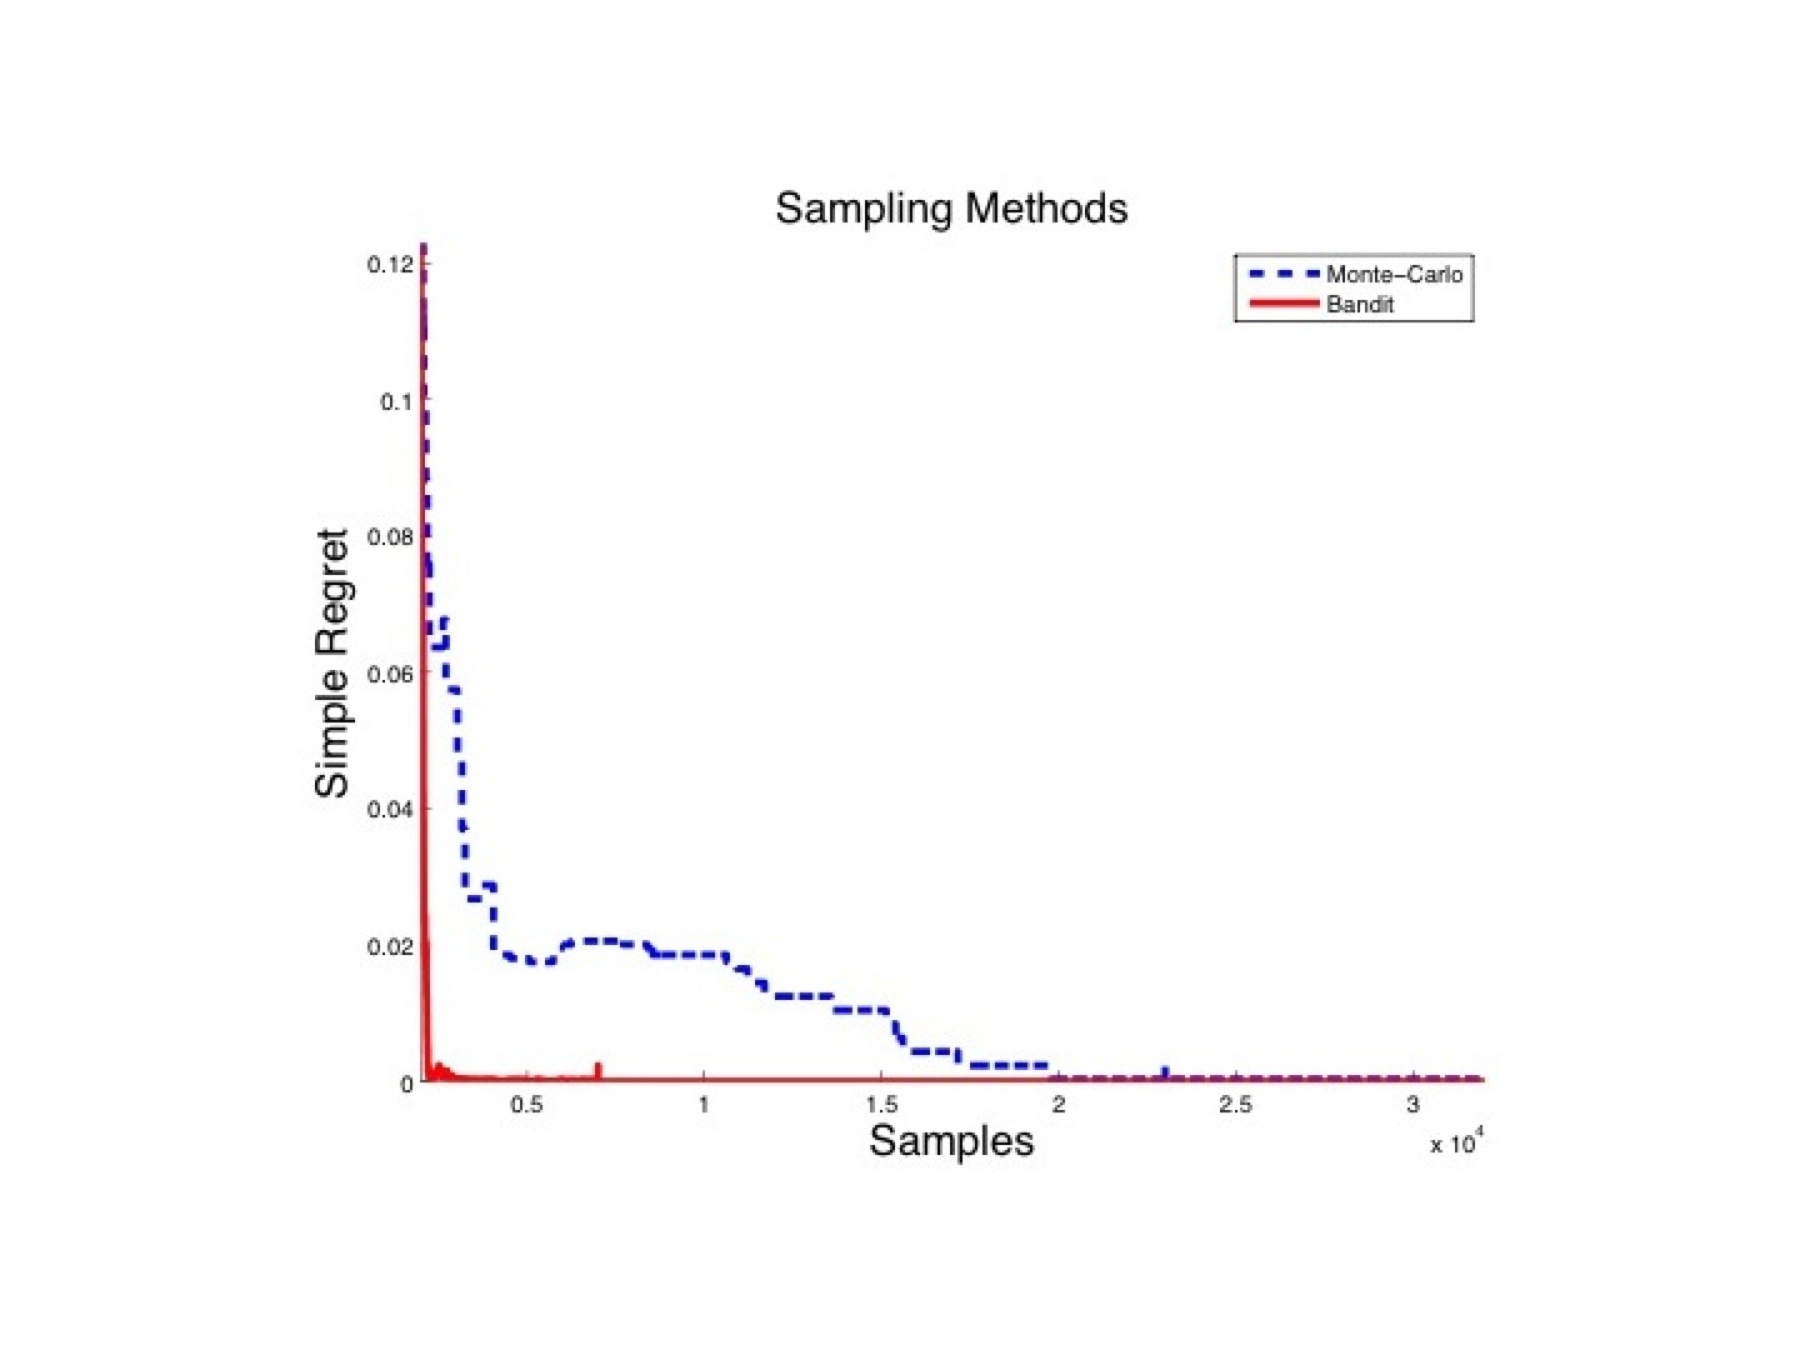
\includegraphics[scale = 0.3]{figures/Slide01.jpg}
\caption{Illustration of a grasp plan $\Gamma$ composed of two lines of action, $\gamma_1(t)$ and $\gamma_2(t)$}
\vspace*{-10pt}
\label{fig:line_of_action}
\end{figure}

\subsection{Problem Definition}

Given a 2-D workspace $\mathcal{W}$, with an unknown object represented as a trained GPIS model (we will describe the GPIS model later) and set of possible grasp plans $G$.
We are interested in determining 

\begin{align}\label{eq:problem_def}
\Gamma^* \in \mbox{argmax}_{\Gamma \in G} E(Q(\Gamma))
\end{align}

with respect to a chosen grasp metric Q. 


\subsection{Multi-Arm Bandits for Grasp Selection}
While a standard approach to solving the problem in Eq. \ref{eq:problem_def} would be to simply perform Monte-Carlo integration on each $\Gamma_i$ and compute the expected grasp quality, we propose treating the problem as a multi-arm bandit problem and forming a policy for selecting which grasp to sample. 
In our setting, we have a probabilistic shape representation and would like to evaluate many potential grasps on that shape model.
Motivated by limited computational resources we are interested in how to intelligently allocate sampling resources to efficiently find the best grasp plan $\Gamma^*$.
Here each arm corresponds to a different grasp plan and pulling the arm is sampling the shape representation and evaluating the arm's grasp plan on the sampled shape representation.
The reward for pulling an arm is the grasp quality of the resulting grasp on the sampled shape.
We have a policy for exploration of different grasp plans (i.e. choosing which one to sample next) and at a given stopping time we choose to execute the grasp plan with the highest expected quality based on the samples received so far, which would correspond to actually performing the grasp.  
The number of samples needed before the simple regret reaches zero, determines how effective an exploration policy is for grasp evaluation.

In solving Eq. \ref{eq:problem_def}, we want to pick the grasp plan with the highest $E(Q(\Gamma))$ determined via Monte-Carlo Integration.
Due to the non-linear nature of our grasp metric, we currently do not have a way to represent the distribution on grasp quality of $p(Q(\Gamma))$ in closed form.
Thus, we are restricted in the type of bandit policies available to us, since most sophisticated polices require distributional information. \todo{double check with Dylan}

For our exploration policy, we maintain a subset of the possible grasp plans that are statistically indistinguishable from the best grasp plan.
During exploration, we sample uniformly from this subset.
This has been shown to have good performance when the number of evaluations is large \cite{bubeck2009pure}.
For each grasp plan, we maintain a $95\%$ confidence interval around the expected quality of the grasp plan.
The width of the confidence interval for a grasp plan $i$ that has been sampled $n_i$ times and the samples have standard deviation $\sigma_i$ is:

\vspace{-2ex}
\begin{align}
C_{ i} := \frac{1.96 \sigma_i}{\sqrt{n_i}}.
\end{align}

Let $\hat{\mu_i}$ be the sample mean of the grasp quality for grasp plan $i$.
Then the confidence interval for grasp plan $i$ is $[\hat{\mu_i} - C_i, \hat{\mu_i} + C_i]$ \cite{caflisch1998monte}.  
After a sample from a grasp plan, we check to see if the confidence interval of the sampled grasp intersects with the confidence interval of the current best grasp plan, and if it does not, we prune that grasp plan from the current active set of  grasp plans. Since we prune grasps that our below a confidence interval we have statistical guarantees unlike earlier approaches to this problem\cite{kehoe2012toward}. In future work, we will look at using other exploration strategies. 




\begin{figure}[ht!]
\centering
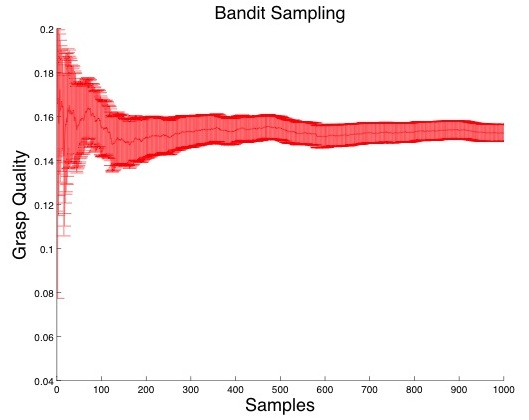
\includegraphics[width=8.5cm,height=9cm]{figures/Slide11.jpg}
\caption{ \footnotesize Convergence of expected grasp quality, $E(Q(g))$,  for a typical grasp. You can see it can take hundreds of evaluations to correctly estimate the expected grasp quality, thus it is important to  intelligently allocate sampling resources}
\vspace*{-10pt}
\label{fig:sampling_convergence}
\end{figure} 



\subsection{Gaussian Process (GP) Background} \todo{massive trim down}
GPs provide an infinite dimensional analogue of Multivariate
Gaussian Distributions which allow us to model distributions over
functions. Gaussian processes (GPs) are widely used in machine learning as a nonparametric regression method for estimating continuous functions from sparse and noisy data \cite{rasmussen2010gaussian}.
In a GP, a training set consists of input vectors $\mX = \{\bx_1, \ldots, \bx_n\}$, $\bx_i \in \mathbb{R}^d$, and corresponding observations $\by = \{y_1, \ldots, y_n\}$. The observations are assumed to be noisy measurements from the unknown target function $f$:
\begin{equation}
y_i = f(\bx_i) + \epsilon,
\end{equation}
where $\epsilon \sim \mN(0,\sigma^2)$ is Gaussian noise in the observations.
A zero-mean Gaussian process is completely specified by a covariance function $k(\cdot,\cdot)$, also referred to as a kernel.
Given the training data $\mD = \{\mX, \by\}$ and covariance function $k(\cdot,\cdot)$, the posterior density $p(f_*|\bx_*,\mD)$ at a test point $\bx_{*}$ is shown to be \cite{rasmussen2010gaussian}:
\begin{align*}
	p(f_*|\bx_*,\mD) &\sim \mN\big(\mu(\bx_*), \Sigma(\bx_*)\big) \\
	\mu(\bx_*) &= k(\mX,\bx_*)^{\intercal}(K + \sigma^2I)^{-1}\by \\
	\Sigma(\bx_*) &= k(\bx_*,\bx_*)-k(\mX,\bx_*)^{\intercal}(K+\sigma^2I)^{-1}k(\mX,\bx_*)\big) 
\end{align*}
where $K \in \mathbb{R}^{n \times n}$ is a matrix with entries $K_{ij} = k(\bx_i,\bx_j)$ and $k(\mX,\bx_*) = [k(\bx_1,\bx_*),\ldots,k(\bx_n,\bx_*)]^{\intercal}$. 
This derivation can also be used to predict the mean and variance of the function gradient by extending the kernel matrices using the identities \cite{solak2003derivative}:

\vspace{-2ex}
\begin{align}
	\text{cov}\left(f(\bx_i), f(\bx_j) \right) &=  k(\bx_i, \bx_j) \\
	\text{cov}\left(\frac{\partial f (\bx_i)}{\partial x_k}, f(\bx_j) \right) &= \frac{\partial}{\partial x_k} k(\bx_i, \bx_j) \label{eq:mean_gradient}\\
	\text{cov}\left(\frac{\partial f (\bx_i)}{\partial x_k}, \frac{\partial f (\bx_j)}{\partial x_l} \right) &= \frac{\partial^2}{\partial x_k \partial x_l} k(\bx_i, \bx_j)\label{eq:cov_gradient}
\end{align}

\begin{figure}[ht!]
\centering
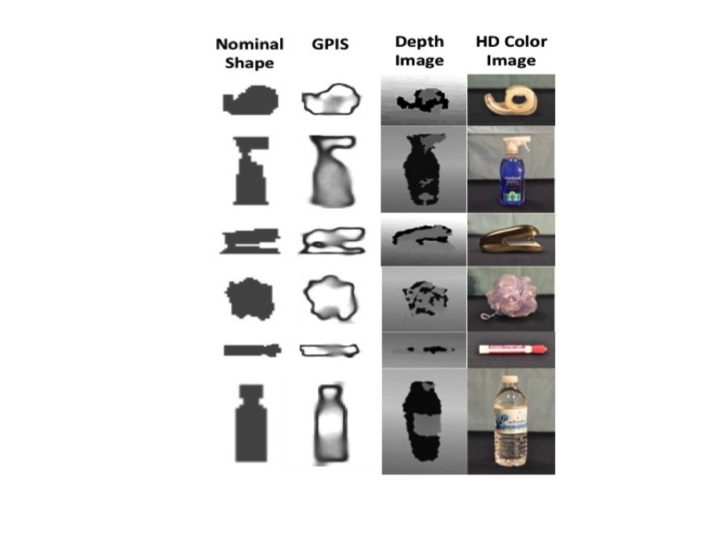
\includegraphics[width = 8.5cm, height = 14cm ]{figures/Slide03.jpg}
\caption{\footnotesize Six example objects illustrating transparency, specularity, sensor noise that illustrate the need for shape uncertainty: (from top to bottom) tape, squirt bottle, stapler, loofa, marker, water bottle. Displayed from right to left are the HD color image, a point cloud observation from a Primesense Carmine, GPIS visualization technique from \cite{jeffs}, the nominal shape on a $25 \times 25$ grid.  }
\vspace*{-10pt}
\label{fig:GPIS_TSDF}
\end{figure}
%\section{Related Work}

For our kernel choice we decided to use the square exponential kernel, a major reason for this was its differentiability. Other kernels relevant to GPIS are the thin-plate splines kernel and the Matern kernel \cite{williams2007}. 

We construct a GPIS by learning a Gaussian Process to fit measurements of a signed distance field of an unknown object.  Precisely, $x_i \in \mathbb{R}^2$ in 2D and $x_i \in \mathbb{R}^3$ in 3D, and $y_i \in \mathbb{R}$ is a noisy signed distance measurement to the unknown object at $x_i$.







\section{Evaluating a Grasp}
 In order to solve our problem definition, we must evaluate $E(Q(\Gamma))$ for a given grasp plan $\Gamma$. We will first discuss which grasp metric $Q$ we chose and then proceed into evaluating the expectation $E$ efficiently. 

\subsection{Grasp Metric}
In their pioneering work over two decades ago Ferrari and Canny \cite{ferrari1992}, demonstrated a method to rank grasps by considering their contact points and surface normals. Importantly the magnitude of Q yields a measurement that allows one to rank grasps by their physical stability and evaluate the property of force-closure. Furthermore, it has wide spread use in grasp packages like GraspIT\cite{miller2004graspit}, OpenGrasp\cite{73} and Simox \cite{vahrenkamp2010simo}, which motivates studying its effect with uncertainties. 

The $L^1$ version of the metric works by taking as input the contact points $\textbf{c}_1,...,\textbf{c}_m$, surface normals $\textbf{n}_1,...,\textbf{n}_m$, center of mass $z$ and friction coefficient $\mu$. Then constructing a convex hull around the wrenches made up of those parameters and finding the radius of the largest unit ball centered at the origin in wrench space. A wrench is defined as concatenation of a force and torque vector.  If the convex hull doesn't enclose the origin, the grasp is not in force-closure. Thus a grasp can be parameterized by the following tuple $g = \lbrace \textbf{c}_1,...,\textbf{c}_m,\textbf{n}_1,...,\textbf{n}_m,\mu, \textbf{z} \rbrace$, our method is applicable to all grasp metrics that represent a grasp as the tuple $g$, such as \cite{christopoulos2007handling}, \cite{li1988task}. 

\subsection{Calculating the Expected Grasp Quality}
Given a proposed grasp plan $\Gamma$, the expected grasp quality can be evaluated as follows:

\vspace{-2ex}
\begin{align}\label{eq:shape_sampling}
E(Q(\Gamma)) = \int Q(g|S,\Gamma) p(S) dS
\end{align}



Where $Q(g|S,\Gamma)$ is the grasp quality that is computed on a shape sample drawn from $p(S)$. To compute this we intersect the zero crossing of the level set with the propose grasp plan $\Gamma$ and determine the parameters $g$, this has been the approach taken in previous work  \cite{kehoe2012estimating}, \cite{kehoe2012toward},  \cite{christopoulos2007handling}. See Fig. \ref{fig:shape_samples} for an example of what samples drawn from $p(S)$ induced by GPIS look like. For computational reasons we approximate the integral via Monte-Carlo Integration. We use importance sampling to draw from the distribution induced by GPIS and calculate the following

\begin{figure}[ht!]
\centering
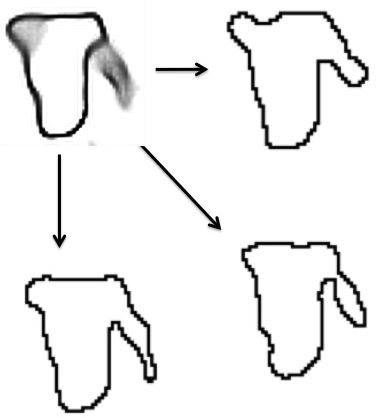
\includegraphics[width = 8.5cm, height= 7cm ]{figures/Slide13.jpg}
\caption{Shape samples drawn from Eq. \ref{eq:joint_shape} on the object in the upper left corner. Given a shape sample we highlight the zero-crossing of the level set in black}
\vspace*{-10pt}
\label{fig:shape_samples}
\end{figure}

\begin{align*}
E(Q(\Gamma)) \approx \frac{1}{N} \sum_{i=1}^N Q(g|S_i,\Gamma) , \ \  S_i \sim p(S)
\end{align*}

To compute the above distribution we must draw samples from $p(S)$. In order to draw shape samples from a GPIS, one needs to sample from signed distance function, $sd$, over the joint on all points in the workspace $\mathcal{W}$ or $p(sd(\mathcal{W}))$. Since this is a GPIS, we know the following 

\begin{align}\label{eq:joint_shape}
p(S) = p(sd(\mathcal{W})) \sim N(\mu(\mathcal{W}),\Sigma(\mathcal{W}))
\end{align}

Thus if the workspace is an $n \times n$ grid, the joint distribution is an  $n^2$ multi-variate Gaussian, due to $sd:\mathbb{R}^2 \rightarrow \mathbb{R}$.  Sampling from a Gaussian involves inverting the covariance matrix and inversion is in the naive way $O(n^3)$ \cite{petersen2008matrix}. Thus the complexity of this operation is $O(n^6)$ in 2D and $O(n^9)$ in 3D. 

To reduce complexity we propose sampling not from the shape distributions, but instead from the distributions on the grasps parameters themselves. We recall that a grasp according to our metric is defined as the tuple $g = \lbrace \textbf{c}_1,...,\textbf{c}_m,\textbf{n}_1,...,\textbf{n}_m,\mu, z \rbrace$. We are thus interested in calculating $p(g|\Gamma,\mu(x),\Sigma(x))$. The distribution on a grasp is defined then as: 

\begin{align}\label{eq:joint_on_shape}
p(g) = p\big(\textbf{c}_1,...,\textbf{c}_m,\textbf{n}_1,...,\textbf{n}_m|\Gamma,\mu(x),\Sigma(x)\big)
\end{align}

We note here that we currently use the friction coefficient $\mu$ and the expected center of mass $\bar{z}$ as deterministic values. For grippers that do not approach along the same line of action (i.e. non-parallel jaw grippers) we make the assumption that each contact and normal pair is independent, or 

\vspace{-2ex}
\begin{align}\label{eq:independence}
p(g) = &\prod_{i=1}^mp\big(\textbf{c}_i,\textbf{n}_i|\gamma_i(t),\mu(x),\Sigma(x)\big)
\end{align}



We compute the expected grasp quality now as follows: 

\vspace{-2ex}
\begin{align}\label{eq:grasp_sampling}
E(Q(\Gamma)) = \frac{1}{N} \sum_{i=1}^N Q(g_i) , \ \ g_i \sim p(g)
\end{align}


We will now show how these distributions can be computed and how the complexity for evaluating a grasp is reduced from $O(n^6)$ to $O(n^3)$. 


\section{Distribution of Grasp Parameters}
\label{sec:distgrasp}
 
 To sample from $p(g)$, we need to sample from the distributions associated with a line of action $p(\textbf{n}_i,\textbf{c}_i|\gamma_i(t),\mu(x),\Sigma(x))$. Using Bayes rule we can rewrite this as 
 
 \vspace{-2ex}
 \begin{align*}
 &p(\textbf{n}_i,\textbf{c}_i|\gamma_i(t),\mu(x),\Sigma(x))=\\
 &p(\textbf{n}_i|\textbf{c}_i,\gamma_i(t),\mu(x),\Sigma(x))p(c_i|\gamma_i(t),\mu(x),\Sigma(x))
 \end{align*}
 
 In section \ref{sec:contact}, we look at how to sample from $p(\textbf{c}_i|\gamma_i(t),\mu(x),\Sigma(x))$. Then in section \ref{sec:normals}, we look at how to sample from $p(\textbf{n}_i|\textbf{c}_i,\gamma_i(t),\mu(x),\Sigma(x))$ and present a novel visualization technique for the distribution on surface normals. Lastly in section \ref{sec:mass}, we show a way to calculate the expected center of mass assuming a uniform mass distribution. 
 .
\subsection{Distribution on Contact Points}\label{sec:contact} 
We would like to find the distribution on contact point $\textbf{c}_i$. A contact point in terms of the GPIS and line of action model can be defined as the point, $t$, when the signed distance function is zero and no points before said point along the line have touched the surface. We express this as the following conditions: 

\vspace{-2ex}
\begin{align}
 &sd(\gamma(t)) = 0 \label{eq:density_cond} \\
&sd(\gamma(\tau)) > 0, \: \forall \tau \in [a,t) \label{eq:cdf_cond}
\end{align}

We will now demonstrate how to efficiently sample from $p(\textbf{c}_i|\mu{x},\Sigma{x},\gamma_i{t})$

The probability distribution along the line $\gamma(t)$ is given by:

\vspace{-2ex}
\begin{equation} \label{eq:line_of_act_dist}
p\big(sd(\gamma(t)) ; \mu(t),\Sigma(t)\big) \ \forall t \in [a,b] 
\end{equation}

This gives the signed distance function distributions along the entire line of action in the workspace as a multivariate Gaussian. One could think of this as a marginalization of all other points in signed distance field except the line of action. To sample contact points, one can simply draw samples from Eq. \ref{fig:line_of_action} and iterate from $a$ to $b$ until they reach a point that satisfies  Eq. \ref{eq:density_cond} and Eq. \ref{eq:cdf_cond}. 

\begin{figure*}[ht!]
\centering
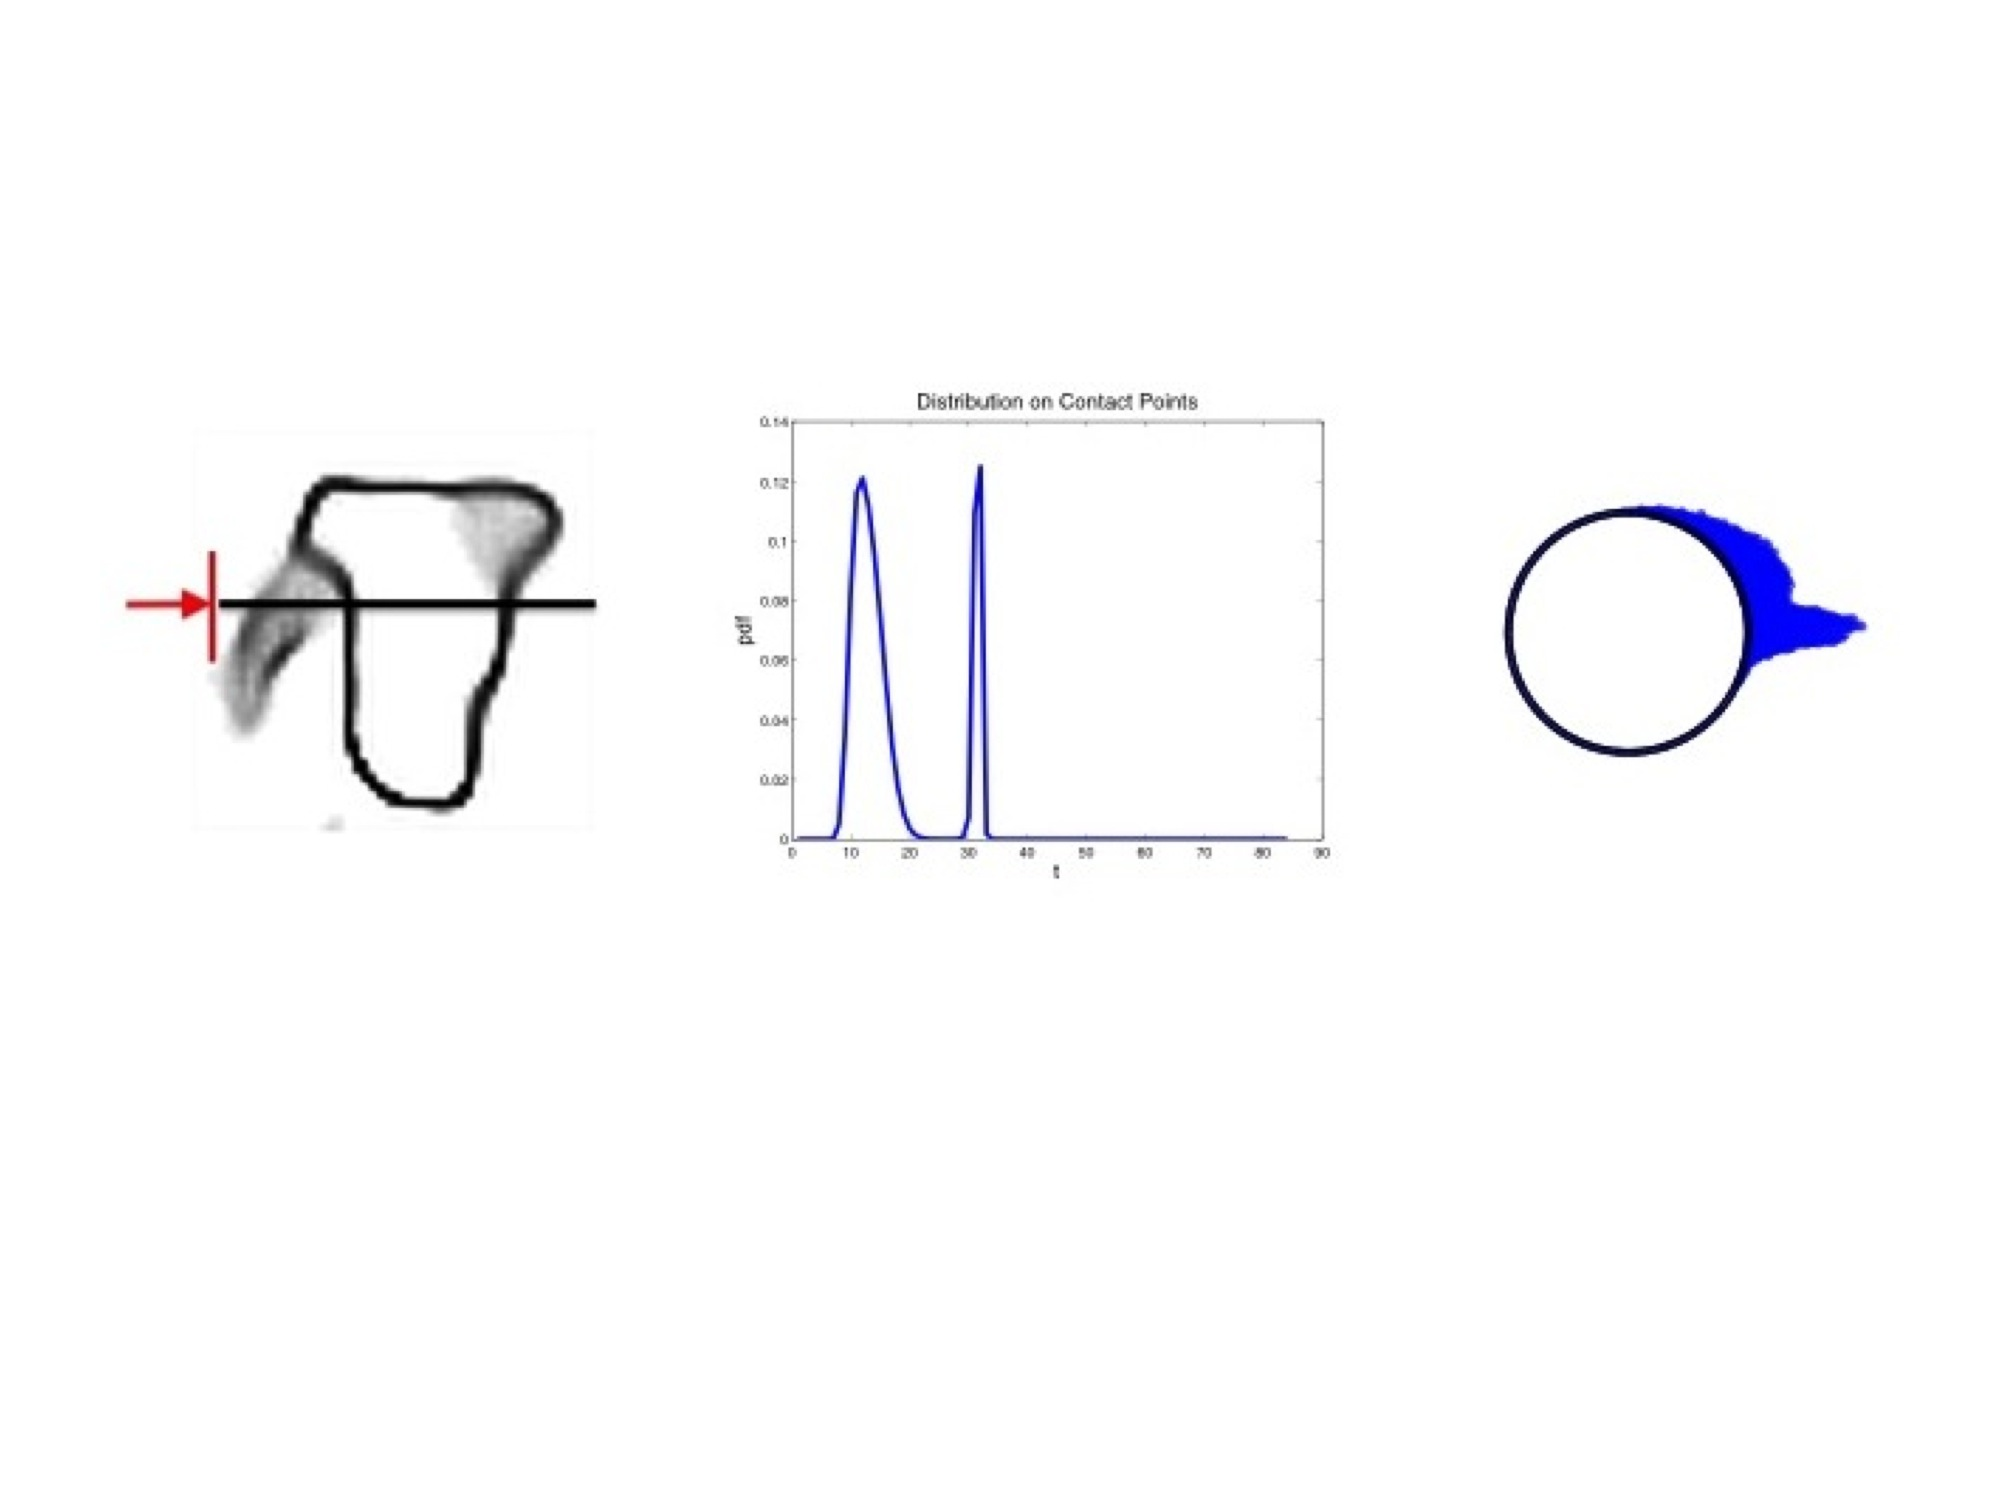
\includegraphics[width = 17cm, height = 4.5cm]{figures/Slide04.jpg}
\caption{ \footnotesize (Left to Right): Line of action for a given gripper on an uncertain surface representing a measuring cup. Distribution $p(c)$ as a function of $t$, the position along the line of action $\gamma(t)$. The two modes correspond to the different potential contact points, either the handle or the base of the cup. Lastly, the distribution on the surface normals (inward pointing) along $\gamma(t)$ described by equation \ref{eq:normal_dist}. }
\vspace*{-10pt}
\label{fig:GraspDist}
\end{figure*}



\subsection{Distribution on Surface Normals}\label{sec:normals} 
Using Eq. \ref{eq:mean_gradient} and Eq. \ref{eq:cov_gradient}, we can compute the mean of the gradient $ \mu_{\nabla}(x)$ and the covariance of the gradient $\Sigma_{\nabla}(x)$ respectively. Thus we can compute the distribution around the surface normal for a given point in $\mathcal{W}$. We can now write 

\vspace{-2ex}
\begin{align*}
p\big(\textbf{n}_i|\textbf{c}_i = \gamma(t)\big) = p\big(\textbf{n}_i |\mu(\gamma(t)), \Sigma(\gamma(t)) \big)
\end{align*}

One interesting effect of this technique is that we can now marginalize out the line of action model and visual what the surface normal distribution is along a given line of action. To our knowledge this is the first attempt to visual surface normals along a grasp plan. Marginalization can be performed as follows:

\vspace{-2ex}
\begin{equation}
p(\textbf{n}_i ) = \int_a^b   p\big(\textbf{n}_i = \textbf{v} | \textbf{c}_i = \gamma(t) \big)p\big(\textbf{c}_i = \gamma(t)\big) dt
\end{equation}

Grasp metrics such as  Ferrari-Canny require $\textbf{n}_i$ be normalized, or, equivalently, a member of the sphere $\mathcal{S}^{d-1}$ \cite{ferrari1992}. To account for this we densely sample from the  distribution $p \big(\textbf{n}_i ) \big)$  and project onto $\mathcal{S}^{d-1}$.  In Fig.\ref{fig:GraspDIst}, we visualize the theoretical distribution on $\textbf{n}_i$ calculated for a given GPIS and approach line of action.


\subsection{Expected Center of Mass}\label{sec:mass} 

We recall the quantity $P(sd(x) < 0) = \int_{-\infty}^{0} p(sd(x) =  s \ | \ \mu(x),\Sigma(x)) ds$ is equal to the probability that $x$ is interior to the surface under the current observations.
We assume that the object has uniform mass density and then $P(sd(x) < 0)$ is the expected mass density at $x$.
Then we can find the expected center of mass as:

\begin{equation}
  \bar{z} 
  =
  \frac
    {\int_{\mathcal{W}}x P(sd(x)<0) dx}
    {\int_{\mathcal{W}}  P(sd(x)<0) dx}
\end{equation}

which can be approximated by sampling $\mathcal{W}$ in a grid and approximating the spatial integral by a sum. Since this operation involves the entire SDF, one would want to use a low resolution grid for computational efficiency. We show the computed density and calculated expected center of mass for a marker in Fig. \ref{fig:GPIS_MASS}.


\begin{figure}[ht!]
\centering
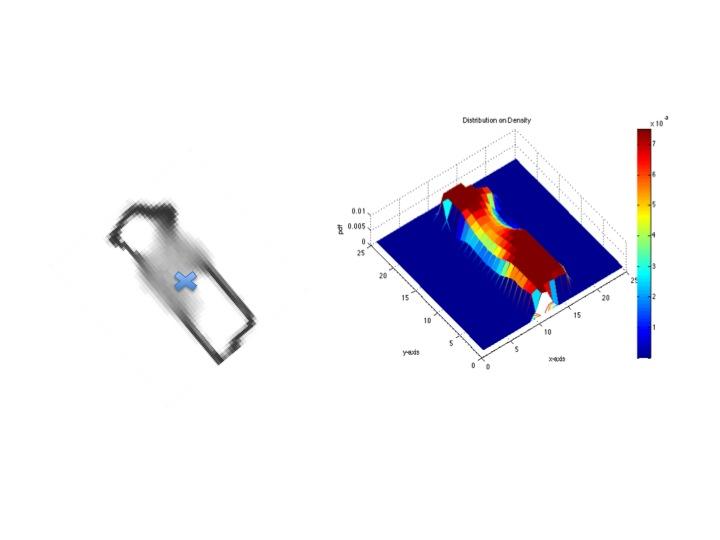
\includegraphics[scale = 0.3]{figures/Slide06.jpg}
\caption{ \footnotesize Left: A surface with GPIS construction and expected center of mass (black X)
Right: The distribution on the density of each point assuming uniform density}
\vspace*{-10pt}
\label{fig:GPIS_MASS}
\end{figure}

\subsection{Complexity Analysis on Sampling From Grasps Distributions}

After formally deriving each distribution,  we can now sample along each line of action $\gamma_i(t)$ from the joint distribution $p(\textbf{c}_i,\textbf{n}_i | \gamma_i(t))$, due to our independence assumption Eq. \ref{eq:independence}. This can be done by drawing samples from Eq. \ref{eq:joint_contact_normal}. and using our projection technique for the normal distribution. 

Having a distribution along a line of action model allows us to sample from those instead of the joint distribution $p(sd(\mathcal{W}))$. Assuming the line of action is on the order of $n$, sampling from this distribution for a single grasp is $O(n^3)$. However, each proposed grasp plan $\Gamma$ requires the distribution to be computed, so if we have $T=|G|$ then the complexity is $O(Tn^3)$. In practice, this should be much smaller than $O(n^6)$. 




\section{Experiments}
For the experiments below we used common household objects shown in Fig. \ref{fig:GPIS_TSDF}. We manually created a 25 x 25 grid, by tracing a pointcloud of the object on a table taken with a Primesense Carmine depth sensor. To accompany the SDF, we created an occupancy map, which holds 1 if the point cloud was observed and 0 if it was not observed, and a measurement noise map, which holds the variance 0-mean noise added to the SDF values. The parameters of the GPIS were selected using maximum likelihood on a held-out set of validation shapes. Our visualization technique follows the approach of \cite{jeffs} and consisted of drawing many shape samples from the distribution and blurring accordingly to a histogram equalization scheme. 

We did experiments for the case of two hard contacts in 2-D, however our methods are not limited to this implementation. We drew random lines of actions $\gamma_1(t)$ and $\gamma_2(t)$ by sampling around a circle with radius $\sqrt{2}n$ and sampling the circles origin, then projecting onto the largest inscribing circle in the workspace. 


\subsection{Sampling from Grasps Vs. Shape}
We first tested 1000 grasp plans and sampled each one 5000 times  and measured the RMS error between converged expected grasp plan qualities for sampling shape Eq. \ref{eq:shape_sampling} vs. grasps  Eq. \ref{eq:grasp_sampling} was 0.004. After confirming the distributions converged close to the same value, we show the computational complexity in Fig. \ref{fig:speed_dif} of the two methods for evaluating 100 grasps on an $n \times n$ grid. 



\begin{figure}[ht!]
\centering
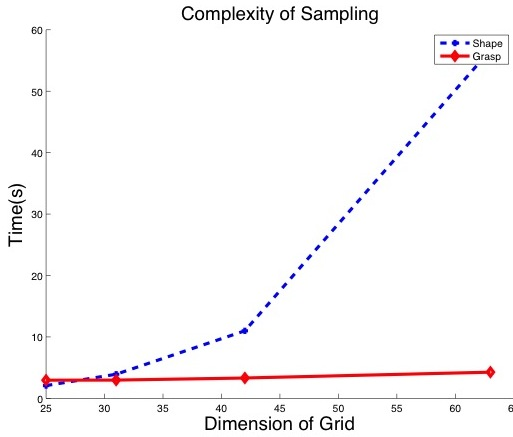
\includegraphics[width=8.5cm,height=9cm]{figures/Slide12.jpg}
\caption{ \footnotesize Time it took to sample from 100 grasp distributions for a given resulution of the workspace. Blue line is sampling from $p(sd(\mathcal{R}))$ or shapes and Green is sampling from $p(g)$ or the calculated distribution on grasps. As you can see sampling from the calculated distributions scales much better. }
\vspace*{-10pt}
\label{fig:speed_dif}
\end{figure}





\subsection{Adaptive Sampling Technique}

We consider the problem of selecting the best grasp out of a set $G$ given a fix number of iterations $I$. For our experiments we look at selecting the best grasp out of a size of $|G| = 1000$ and $I= 7000$ or when the set of grasps is a single grasp. In Fig. \ref{fig:simple_regret}, we plotted the simple regret, Eq. \ref{eq:simple_regret}, averaged over 20 runs and compare it to the naive Monte-Carlo method that randomly chooses a grasp plan to draw a sample from . The most interesting thing is that the regret is minimized an order of magnitude faster than the naive approach, thus motivating the use of including observations as you select samples. 


\begin{figure}[ht!]
\centering
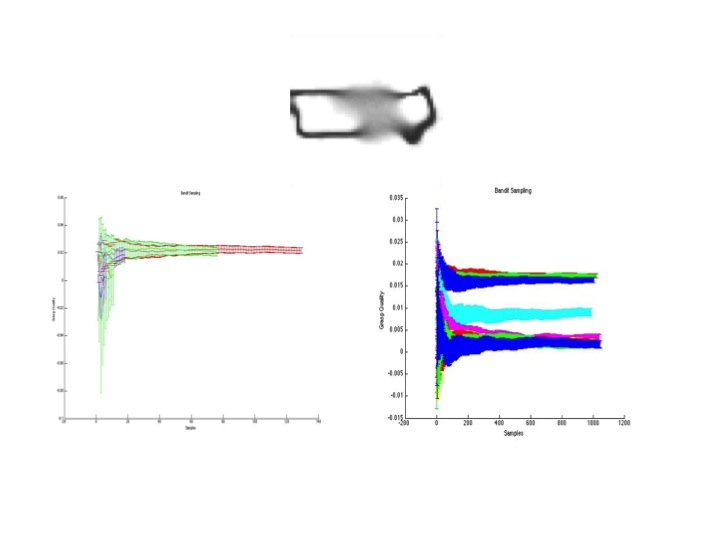
\includegraphics[width=8.5cm,height=9cm]{figures/Slide09.jpg}
\caption{ \footnotesize Comparison of two sampling methods. Green is the adaptive bandit method that actively chooses which one to sample and Blue is the naive Monte-Carlo method. We measure their ability to converge in terms of simple regret Eq. \ref{eq:simple_regret} averaged over 100 runs. We had them determine the best grasp when $|G|=1000$. As you can see our method converges much faster with an average of evaluation of 4 samples per grasp. We start the process though by deterministically evaluating every grasp 2 times to achieve a baseline, which explains the first part of the graph.}
\vspace*{-10pt}
\label{fig:simple_regret}
\end{figure}







\section{Limitations} 
Sampling from our distribution $p(g)$ over $p(S)$ yields a reduction in computationally complexity, but only if the number of grasps one wants to evaluate remains small relative to $n^3$, techniques to ensure this could be to find locally optimal potential grasps using optimization approaches \cite{jeffs}. 

An additional problem is that we only have an expected center of mass and not a distribution on the center of mass. This might prove to be to expensive to compute, however recent work by Panahi et al. showed a way to bound the center of mass for convex parts. Extension of his work to implicit surfaces could be of possible interest \cite{panahi2014bounding}.  

Our budgeted multi-arm bandit approach appears promising, but we still do not know how well it will perform on 3D shapes and large scale grids. Future work will be building an efficient construction of GPIS to scale to 3D. Lastly, we are interested in investigating how well our algorithm works in parallel computing to be used in the cloud computing context. Furthermore, their is a large literature on formulating bandit policies and experimenting with them all will need to be done to see which one works best. 


\section{Future Work}
We have demonstrated how the multi-arm bandit problem can be used to sample grasps with shape uncertainty. However, one could imagine this approach to work with other forms of uncertainity like pose, center of mass, friction coefficient or motion. 

We are interested in seeing how we can apply this to different shape representations other than GPIS like polygonal \cite{kehoe2012estimating} or splines \cite{christopoulos2007handling}. Furthermore, we want to extend this to 3D and see if our simplest bandit method still works well. There are many different methods for exploration policies, so it would be interesting to see how well they perform in 3D as well. 

\section{Conclusion}

We demonstrate how formulation the problem of grasp selection as multi-arm bandit method enables much more efficeint sampling of grasp plans. We applied this to a new method for shape uncertainity, GPIS. While GPIS has been used before for very interesting applications \cite{hollinger2013},\cite{jeff},\cite{dragiev2011} evaluating a grasp on it remained to computationally intensive if one sampled from the distribution on shape, $p(S)$, we present a an alternative distribution to sample from and demonstrate how it reduces computational complexity of sampling. 


\bibliographystyle{ieeetr}
\bibliography{references}

\end{document}
